\documentclass[a4paper, 11pt, oneside]{article}

\usepackage[utf8]{inputenc}
\usepackage[T1]{fontenc}
\usepackage[english]{babel}
\usepackage{array}
\usepackage{shortvrb}
\usepackage{listings}
\usepackage[fleqn]{amsmath}
\usepackage{amsfonts}
\usepackage{fullpage}
\usepackage{enumerate}
\usepackage{graphicx}
\usepackage{alltt}
\usepackage{indentfirst}
\usepackage{eurosym}
\usepackage{titlesec, blindtext, color}
\usepackage[table,xcdraw,dvipsnames]{xcolor}
\usepackage[unicode]{hyperref}
\usepackage{url}
\usepackage{float}
\usepackage{subcaption}
\usepackage[skip=1ex]{caption}
\definecolor{brightpink}{rgb}{1.0, 0.0, 0.5}

\usepackage{titling}
\renewcommand\maketitlehooka{\null\mbox{}\vfill}
\renewcommand\maketitlehookd{\vfill\null}

\newcommand{\ClassName}{ELEN-0060: Information and Coding Theory}
\newcommand{\ProjectName}{Project 2 - Source coding, data compression, and \\ channel coding}
\newcommand{\AcademicYear}{2021 - 2022}

%%%% First page settings %%%%

\title{\ClassName\\\vspace*{0.8cm}\ProjectName\vspace{1cm}}
\author{Maxime Goffart \\180521 \and Olivier Joris\\182113}
\date{\vspace{1cm}Academic year \AcademicYear}

\begin{document}

%%% First page %%%
\begin{titlingpage}
{\let\newpage\relax\maketitle}
\end{titlingpage}

\thispagestyle{empty}
\newpage

%%%%%%%%%%%%%%%%%%%%%%%%%%%%%%%%%%%%%%%%%%

%%% Table of contents %%%
%\tableofcontents
%\newpage

%%%%%%%%%%%%%%%%%%%%%%%%%%%%%%%%%%%%%%%%%%

% CONTENT %
\section{Implementation}

% Implement a function that returns a binary Huffman code for a given probability
% distribution. Give the main steps of your implementation. Verify your code on
% Exercise 7 of the second exercise session (TP2), and report the output of your code
% for this example. Explain how to extend your function to generate a Huffman code of
% any (output) alphabet size.
\subsection{Question 1}
\paragraph{}Our implementation is based on a data structure representing a Node of the tree which has 4 fields: 
\begin{itemize}
\item the symbol of the Node which is 'None' if the Node is not a leaf.
\item the probability of the Node.
\item a pointer to the left child of the Node which is 'None' if the Node is a leaf.
\item a pointer to the right child of the Node which is 'None' if the Node is a leaf.
\end{itemize}

We first create a node for each letter in which we store its symbol, its probability, and 'None' for both children.
Then, we build the tree as seen in class: we iteratively link the two nodes with the lowest probabilities until the tree is complete with a node having 1 as probability at root. Each new node born from the birth of two nodes has for probability the sum of the probabilities of these nodes. It also maintains a link to these two nodes becoming its children, and has for symbol 'None'.
Finally, we recursively build the Huffman code on the basis of the previously built tree and a choice to represent a left child by a 0 and a right child by a 1.

\paragraph{}The output of our code for this question is: \texttt{\{'A': '000', 'B': '001', 'E': '01', 'C': '100', 'D': '101', 'F': '11'\}} which is not
the same as the one found during the exercise session. It is not a problem because the Huffman code is not unique. Our code is acceptable and its tree can be observed in the figure \ref{fig:huffman_tree}.

\begin{figure}[H]
    \center
    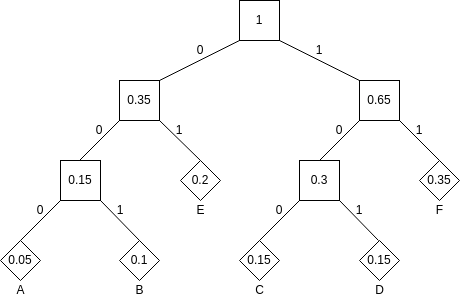
\includegraphics[scale=0.7]{huffman_tree.png}
    \caption{Huffman tree corresponding to the output code}
    \label{fig:huffman_tree}
    \end{figure}

\paragraph{}To generate a Huffman code of any (output) alphabet size, several changes would be necessary both in our data structure and in our algorithm:
\begin{itemize}
    \item Data structure
        \begin{itemize}
            \item We would need to add a field to store the alphabet size $N$ which was implicitly set to 2 in the binary Huffman code.
            \item We would need to store the $N$ children of each node which is not a leaf instead of the two children in the binary Huffman code.
        \end{itemize}
    \item Algorithm
        \begin{itemize}
            \item We would need to take the $N$ lowest probability and link them to create new nodes instead of the two nodes with the lowest probability in the binary Huffman code.
            \item We would need to assign a given unique symbol of the code to each child of a node when recursively building the Huffman code instead of 1 and 0 in the binary Huffman code where there were only 2 children per node.
            \item We might have to deal with problems of number of symbols and size of the alphabet not compatible unlike in the binary Huffman code where it is always possible to merge the two lowest probable nodes. 
        \end{itemize}
\end{itemize}

\subsection{Question 2}

\paragraph{}The example given in the course about state of the art in data compression on slide 50/53 where the sequence 1011010100010 is encoded gives this output for our \texttt{LZ\_online} function:
\begin{itemize}
    \item Dictionary: \{'': (0, ''), '1': (1, '1'), '0': (2, '00'), '11': (3, '011'), '01': (4, '101'), '010': (5, '1000'), '00': (6, '0100'), '10': (7, '0010')\}
    \item Encoded sequence: 100011101100001000010
\end{itemize}

\subsection{Question 3}
\paragraph{}The basic version has one main problem which is address coding. It needs to know the
size of the dictionary before an address encoding. The on-line version solves this problem by using the current dictionary size to determine the number of bits which is equal to $\lceil\log_2{N}\rceil$, where $N$ is the dictionary size. It is thus decreasing the size of the encoded text. This on-line variant is most of the time not very competitive in
terms of optimality but is very robust because it does not need assumptions about source behaviour and can thus allow an instantaneous coding without having to browse the dictionary multiple times. The asymptotic performances are reached only when the dictionary starts to become
representative: when it contains a significant fraction of sufficiently long typical messages.

\subsection{Question 4}
\paragraph{}Running the example given in Figure 2 with our function and taking a \texttt{window\_size} of size 7 gives us this output: "00a00b00r31c21d74d". We have chosen to set the size of the look ahead buffer to the size of the window because it allows to have longer matches prefix and the prefix cannot be longer than the this size.

%%%%%%%%%%%%%%%%%%%%%%%%%%%%%%%%%%%%%%%%%%
\section{Source coding and reversible data compression}

\subsection{Question 5}
\paragraph{}First, we can compute the marginal probability distribution of all the symbols based on the given Morse text. The distribution is:
\begin{table}[H]
    \centering
    \begin{tabular}{|c|c|c|c|c|}
    \hline
    \textbf{Symbol}      & . & - & \_ & / \\ \hline
    \textbf{Probability} & 0.43378 & 0.28706 & 0.21452 & 0.06464 \\ \hline
    \end{tabular}
    \caption{Marginal probability distribution of all the symbols}
\end{table}
Based on the distribution of probabilities, we can compute the binary Huffman code. We get the following code:
\begin{table}[H]
    \centering
    \begin{tabular}{|c|c|c|c|c|}
    \hline
    \textbf{Symbol}      & . & - & \_ & / \\ \hline
    \textbf{Huffman code} & 0 & 11 & 101 & 100 \\ \hline
    \end{tabular}
    \caption{Binary Huffman code}
\end{table}
By applying the obtained Huffman code to the Morse text, we get the encoded Morse text whose size is 2213141 bits. The original Morse text has a size of 2398580 bits. Thus, we have a compression rate of 1.08379.

%%%%%

\subsection{Question 6}
\paragraph{}We can compute the expected average length of the Huffman code by computing the sum for the 4 symbols of the probability of each symbol times the length of the code associated with the symbol.
We get that the expected average length is equal to 1.84538.\\
By comparing to the empirical average length of the Huffman code, we get:
$$\text{Length of encoded } / \text{ length of initial text} = 1.84538$$
This value is the same as the one for the expected average length which is logical since the expected average length was computed based on the probabilities of occurrence of each symbol based on the given Morse text.\\
By comparing to the theoretical bounds, we get that:\\
\begin{equation}
    \frac{H(S)}{log_2(q)} \leq \overline{n} \leq \frac{H(S)}{log_2(q)} + 1$ because $1.77138 \leq 1.84538 \leq 2.77138
\end{equation}
Thus, our code is optimal, because the inequation is satisfied, which was expected because Huffman codes are optimal. But, the obtained code is not absolutely optimal because $\frac{H(S)}{log_2(q)} \neq \overline{n}$.

%%%%%

\subsection{Question 7}
\paragraph{}For the evolution of the empirical average length of the Huffman code with respect to the lengths of the input texts, we get the following plot:
\begin{figure}[H]
    \centering
    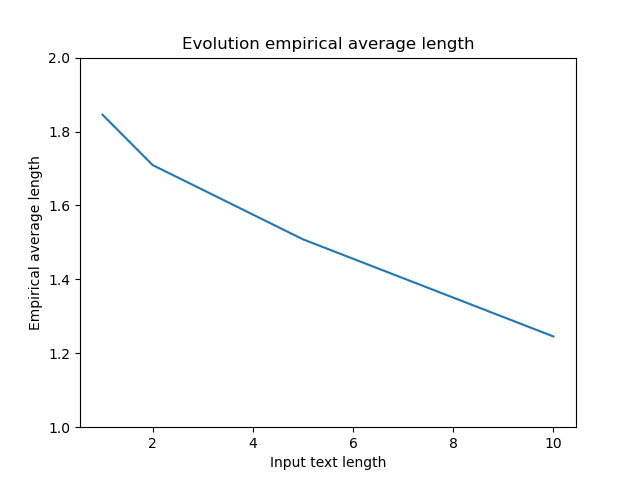
\includegraphics[scale=0.5]{q7.png}
    \caption{Evolution of empirical average length}
\end{figure}
As we can observe on the plot, the empirical average length decreases as the length of the input text increases.

%%%%%

\subsection{Question 8}
\paragraph{}By using the online Lempel-Ziev algorithm to encode the Morse code, we get an encoded code with a total length of 1866281 bits.
The original Morse code has a size of 2398580 bits. Thus, we get a compression rate of $1.28522 = \frac{2398580}{1866281}$.

%%%%%

\subsection{Question 9}
\paragraph{}By using LZ77 to encode the text, we get an encoded text with a total length of 2190809 bits.
The original text has a size of 3060625 bits. Thus, we get a compression rate of 0.673572.

%%%%%

%%%%%
\subsection{Question 10}
\paragraph{}The two algorithms tackle the compression problem using different strategies. The Huffman 
algorithm is based on the frequency of each symbol whereas the LZ77 algorithm is based on referencing of 
redundancy in previous blocks of symbols in the sequence. It is why the combination of these two algorithms can increase the compression rate according to the one obtained by using them alone.
To combine these two algorithms we would first apply the LZ77 algorithm which has as purpose to detect the most redundant group of letters. We think it is better to first
use the LZ77 algorithm because it might have group of letters which are the most frequent and that are not composed of the most frequent letters. For example, in the english language, the 
most frequent letter is 'e' and the second most frequent letter is 't' but the most frequent group of two letters 'th'. Letter-oriented Huffman is good at detecting and compressing files using the letter frequencies alone, but it cannot detect correlations between consecutive letters.
Then we would apply Huffman on the sequence compressed using the LZ77 algorithm. 

\paragraph{}In general, most data compression algorithms are using these 2 parts. First they run the original data through one or multiple transformations typically highly tuned to the particular kind of redundancy in the particular kind of data being compressed like JPEG is doing or tuned to the limitations of human perception like MPEG is doing. Next they run the intermediate data through a single "entropy coder" like Huffman coding.

\subsection{Question 11}
\paragraph{}The length of encoded morse text is equal to 2769551 bits and the compression rate is thus equal to 0.866053739396747.

\subsection{Question 12}

\paragraph{}The values we obtained for the comparison of the lengths and compression rates of the encoded morse text according to the window size are in the table \ref{table:comparison}.

\begin{table}
    \begin{tabular}{|l|l|l|l|l|}
    \hline
    \textbf{Window size} & \textbf{LZ77 length} & \textbf{Huffman-LZ77 length} & \textbf{LZ77 CR} & \textbf{Huffman-LZ77 CR} \\ \hline
    1                    & 3965216 bits         & 2574093 bits                 & 0.6049052561071074             & 0.9318155948522451                     \\ \hline
    1001                 & 2703888 bits         & 2227673 bits                 & 0.8870855597569131             & 1.0767199674278944                     \\ \hline
    2001                 & 2564544 bits         & 2103336 bits                 & 0.9352851813031868             & 1.1403693941433988                     \\ \hline
    3001                 & 2580890 bits         & 2038045 bits                 & 0.9293615768203992             & 1.1769023745795604                     \\ \hline
    4001                 & 2454972 bits         & 1992454 bits                 & 0.9770294732485747             & 1.203832058356178                      \\ \hline
    5001                 & 2546684 bits         & 1957754 bits                 & 0.9418443748812181             & 1.225169250069212                      \\ \hline
    6001                 & 2469908 bits         & 1928162 bits                 & 0.971121191558552              & 1.2439722388471508                     \\ \hline
    7001                 & 2407188 bits         & 1903170 bits                 & 0.9964240433235793             & 1.2603078022457268                     \\ \hline
    8001                 & 2355836 bits         & 1882121 bits                 & 1.0181438775874043             & 1.274402655302183                      \\ \hline
    9001                 & 2478390 bits         & 1864961 bits                 & 0.9677976428245756             & 1.2861287715936152                     \\ \hline
    10001                & 2435940 bits         & 1848255 bits                 & 0.9846630048359155             & 1.2977538272586846                     \\ \hline
    11001                & 2400840 bits         & 1840006 bits                 & 0.9990586628013529             & 1.3035718361787951                     \\ \hline
    \end{tabular}
    \caption{Comparison of the lengths and compression rates of the encoded morse text according to the window size.}
    \label{table:comparison}
    \end{table}
    

\paragraph{}To make easier the comparison between the lengths and compression rates of the encoded morse text, a graphic is represented on the figures \ref{fig:length_comparison} and \ref{fig:compression_rate_comparison}.

\begin{figure}[H]
\center
    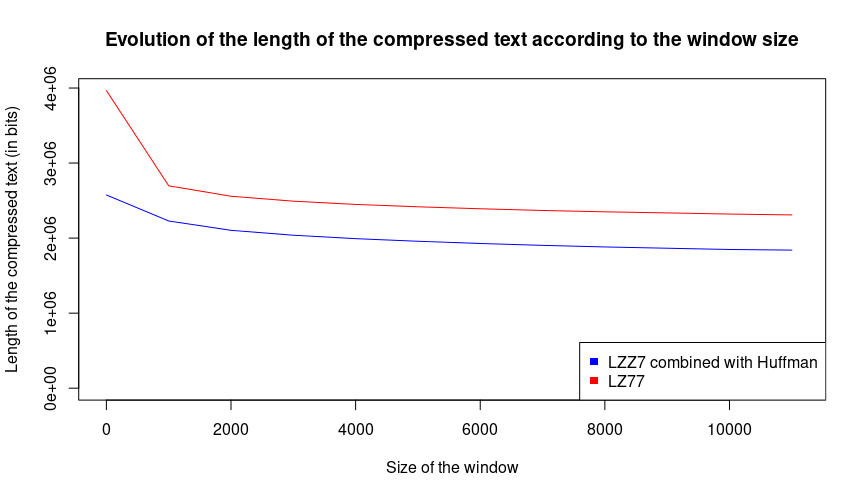
\includegraphics[scale=0.7]{length_comparison.png}
    \caption{Comparison of the length of the encoded morse text according to the window size.}
    \label{fig:length_comparison}
    \end{figure}

\begin{figure}[H]
    \center
    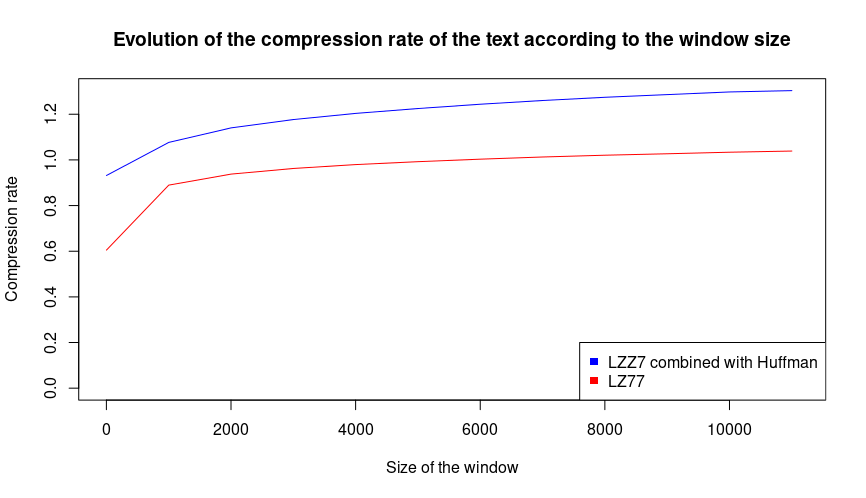
\includegraphics[scale=0.7]{compression_rate_comparison.png}
    \caption{Comparison of the compression rate of the encoded morse text according to the window size.}
    \label{fig:compression_rate_comparison}
    \end{figure}

\paragraph{}We observe that we have better result when combining LZ77 with Huffman than when using LZ77 alone. Moreover, in both case the length is decreasing and the compression rate is increasing when the window size is increasing.
One of the problem of LZ77 is that we might have reserved a lot of bits for the two first values of one LZ77 triplet. Indeed, these values requires at most $\lceil\log_2({\texttt{window\_size + 1})}\rceil$ bits to be encoded but we do not know in advance the amount of bits we will need and we thus reserve this amount of bits. It is especially a drawback for large window sizes: we are reserving $\lceil\log_2({\texttt{window\_size + 1})}\rceil$  bits for these values but
if we have not a long repeating sequence, the majority of the most significant bits we have reserved will be set to 0 which corresponds to useless information. Huffman applied after LZ77 needs the frequency of the triplets computed by LZ77 
and can after increases the compression rate by reducing the number of bits used to encode the triplets.

\paragraph{}As computed in the question 8, LZ online leads to a compressed sequence of length 1866281 bits which corresponds to a compression rate of 1.28522 which are better results than the ones we obtained using LZ77 but not when combining LZ77 and Huffman and taking a window of 11000.
It should be due to the fact that the purpose of this algorithm is to use an online number of bits in opposite to LZ77 which might reserved useless bits as explained previously.

\subsection{Question 13}
\paragraph{}In order to increase the compression rate, we could consider a modified Huffman algorithm for which, instead of considering individual letters, we would consider
entire words. Thus, more frequent words would be assigned shorter codes whereas less frequent words would be assigned longer codes.
So, it would further increase the compression rate.

\paragraph{}Another idea could be to use LZ77 using a large window size as it is one of its main purpose and then apply Huffman on the output of the first algorithm.
This implementation has been studied in the previous question and gave us the best result on a standard morse text. Thus, if we have frequent repetition of words with 
a large distance, this algorithm will lead to better results.

\subsection{Question 14}
\paragraph{}By computing the Huffman code on the original (27 symbols) text, we get the following code:
\begin{table}[H]
    \centering
    \begin{tabular}{|c|c|c|c|c|c|c|c|}
    \hline
    \textbf{Symbol} & \textbf{a} & \textbf{b} & \textbf{c} & \textbf{d} & \textbf{e} & \textbf{f} & \textbf{g} \\ \hline
    \textbf{Code}   & 1010       & 100000     & 100010     & 11010      & 001        & 100011     & 00000      \\ \hline
    \textbf{Symbol} & \textbf{h} & \textbf{i} & \textbf{j} & \textbf{k} & \textbf{l} & \textbf{m} & \textbf{n} \\ \hline
    \textbf{Code}   & 0111       & 0100       & 1100111001 & 1100110    & 11000      & 110010     & 0110       \\ \hline
    \textbf{Symbol} & \textbf{o} & \textbf{p} & \textbf{q} & \textbf{r} & \textbf{s} & \textbf{t} & \textbf{u} \\ \hline
    \textbf{Code}   & 1001       & 100001     & 1100111011 & 0101       & 0001       & 1011       & 00001      \\ \hline
    \textbf{Symbol} & \textbf{v} & \textbf{w} & \textbf{x} & \textbf{y} & \textbf{z} & \textbf{}  & \textbf{}  \\ \hline
    \textbf{Code}   & 11001111   & 110110     & 1100111010 & 110111     & 1100111000 & 111        &            \\ \hline
    \end{tabular}
    \caption{Binary Huffman code for original text}
\end{table}
The expected average length of the code is 4.15047 and the experimental length of the encoded text is 1711279 bits.\\
The original text has a size of 2061550 bits and the encoded text has a size of 1711279 bits. Thus, the compression rate is 1.2046 (= 2061550/1711279).

%%%%%

\subsection{Question 15}
\paragraph{}By comparing the values obtained at the questions 5 and 14, we can conclude that it is better to encode
directly the text without first converting it to Morse because the size of the encoded Morse text is 2213141 bits
while the size of the encoded text is 1711279 bits. Furthermore, the compression rate obtained is higher in question 14
compared to question 5.\\
This can be justified theoretically by the fact that using Huffman encoding with 27 symbols instead of 4 symbols allows to
benefit more from the frequencies of letters in English. For instance, the letter z in English is way less frequent
than the letter e. While using the Morse encoding, the 2 symbols . and - both appear for some of the letters. Thus, we
loose the benefit provided by less frequent letters that will get longer codes and more frequent letters will get shorter codes.

%%%%%%%%%%%%%%%%%%%%%%%%%%%%%%%%%%%%%%%%%%
\section{Channel coding}

\subsection{Question 16}
\paragraph{}In order to implement a function to read and display the given image, we used the methods \texttt{imread} and \texttt{imshow} provided by OpenCV.

%%%%%

\subsection{Question 17}
\paragraph{}To encode the image signal, we used a fixed-length binary code of 8 bits. We have chosen 8 bits because there are 256 (from 0 to 255) possible values, so we need $\lceil log_2(256) \rceil =8$.\\
The code is the binary representation of the grayscale value of each pixel.

%%%%%

\subsection{Question 18}
\paragraph{}By simulating the channel effect on the binary signal of the image, we get the following image:
\begin{figure}[H]
    \centering
    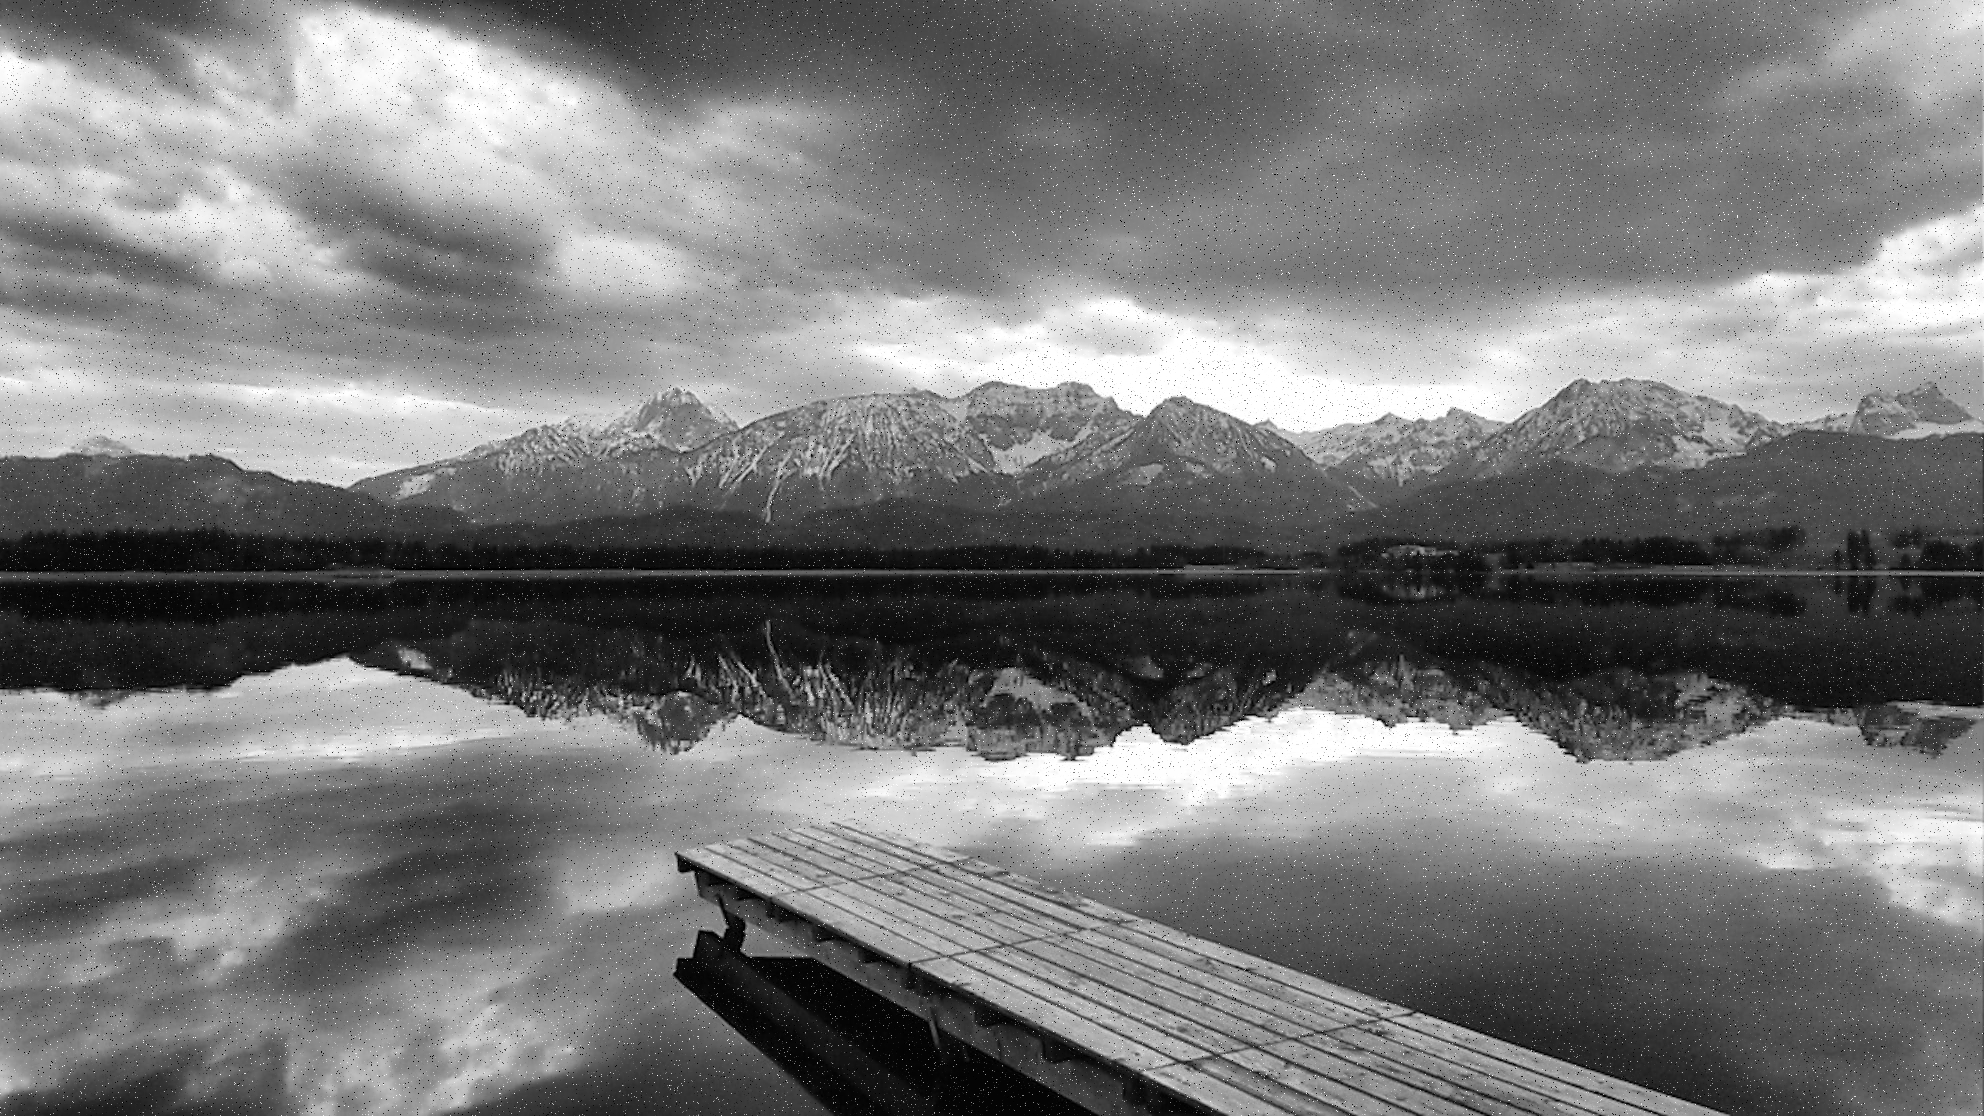
\includegraphics[scale=0.2]{q18.png}
    \caption{Image after simulating the channel effect}
\end{figure}
As we can see in the picture, after simulating the channel effect, there are a lot of small dots\footnote{Zoom in the image to see them better.} that are pixels with different grayscale values
compared to their very close neighbors.\\
This is due to the fact that we are simulating a potential loss bit by bit and we are not using any sort of redundancy.
Thus, if one of the most significant bits is modified, it completely changes the grayscale value for the pixel.

%%%%%

\subsection{Question 19}
\paragraph{}In order to compute the Hamming(7,4) code for the binary image signal, we need to add 3 redundancy bits for every 4 bits. The 3 redundancy bits are:
\begin{itemize}
    \item Bit 1 = $(bit 0 + bit 1 + bit 2) \ mod \ 2$
    \item Bit 2 = $(bit 1 + bit 2 + bit 3) \ mod \ 2$
    \item Bit 3 = $(bit 0 + bit 2 + bit 3) \ mod \ 2$
\end{itemize}
where bit 0, bit 1, bit 2, and bit 3 are, respectively, the first, second, third, and fourth bits for which we want to add redundancy.\\
By applying this principle on each block of 4 bits from the binary image signal, we get the Hamming(7,4) code for the entire binary image signal.

%%%%%

\subsection{Question 20}
\paragraph{}If we decode the binary image signal with redundancy, we get the following image:
\begin{figure}[H]
    \centering
    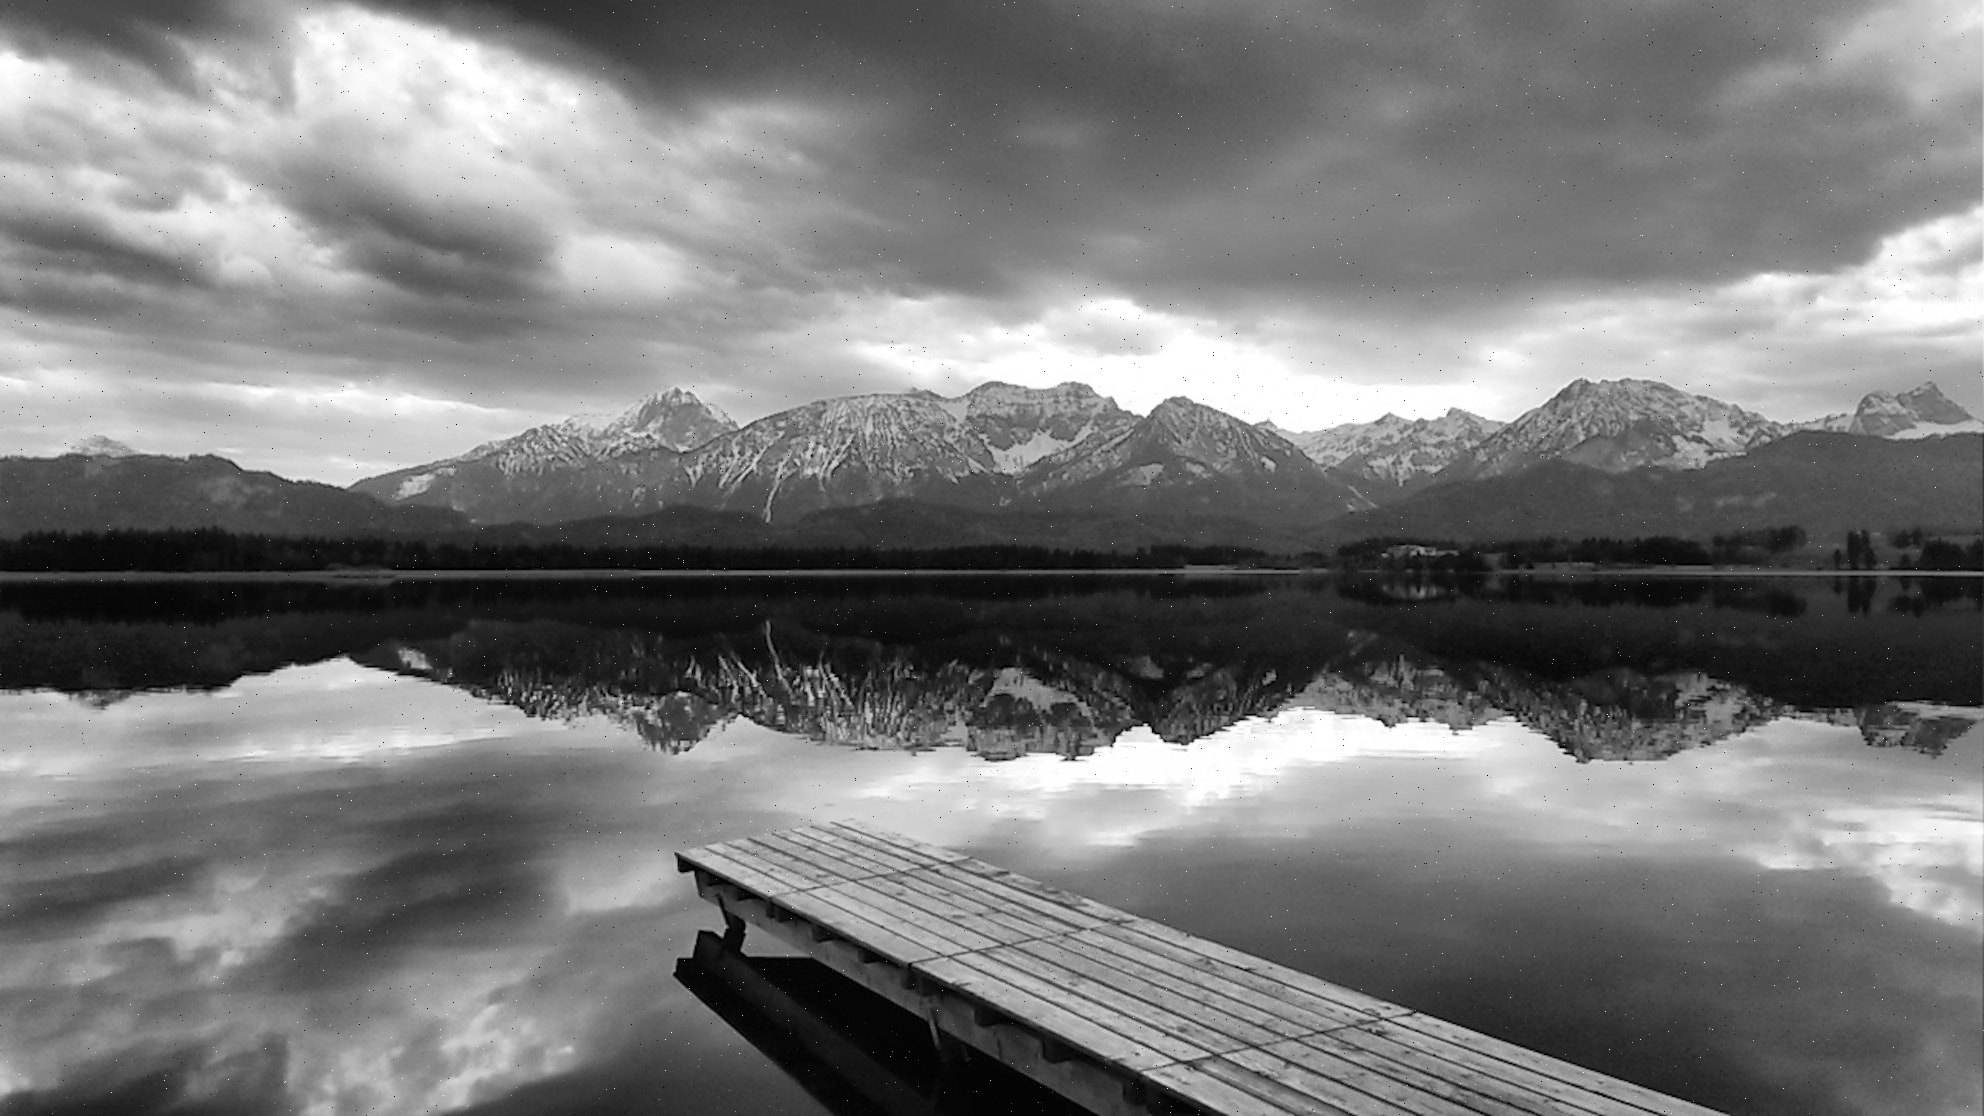
\includegraphics[scale=0.2]{q20.png}
    \caption{Image after simulating the channel effect with redundancy}
\end{figure}
As we can see in the picture, we observe less dots compared to \textit{question 18}. This is because we used redundancy with the Hamming(7,4) code.
Yet, we can still observe some dots. This is because Hamming(7,4) code can correct only one error per chunk of bits. In some cases, we might have more
than one error per chunk thus the original source is not recoverable.
\paragraph{}In order to decode the binary signal with redundancy, we used the syndrome decoding technique, as in the exercise sessions.\\
To apply this technique, we consider that the source bits were correctly transmitted through the channel. Then, we recompute the 3 parity bits based on the received 4 source bits.
Afterwards, we apply a bitwise and between the received parity bits and the re-computed parity bits.\\
Based on the result of the bitwise operation, multiple cases are possible:
\begin{itemize}
    \item If 2 or 3 bits are 1 in the result of the bitwise operation, we can deduce that one of the source bit has been incorrectly transmitted.
    To recover from the error, we can proceed the following way:
        \begin{itemize}
            \item If bits 0 and 1 of the bitwise and are 1, we need to flip the second source bit.
            \item If bits 1 and 2 of the bitwise and are 1, we need to flip the fourth source bit.
            \item If bits 0 and 2 of the bitwise and are 1, we need to flip the first source bit.
            \item If all the bits of the bitwise and are 1, we need to flip the third source bit.
        \end{itemize}
    \item If 1 bit is 1 in the result of the bitwise operation, we can deduce that one of the parity bit has been incorrectly transmitted.
    \item It is possible that 2 or more bits were transmitted incorrectly. In that case, we cannot recover from the error.
\end{itemize}

%%%%%

\subsection{Question 21}
\paragraph{}In order to reduce the loss of information, we could use Reed-Solomon codes instead of Hamming(7,4) because they allow to correct more than 1 errors
in some situations.\\
Another solution is to replace the type of channel. For instance, replacing copper wire with fiber optic in computer networks.
But, it is not also feasible.\\
There is always a trade-off between the rate and the capability of correcting from errors. Thus, in order to increase the rate,
we would need to decrease the redundancy introduced for parity.

%%%%%%%%%%%%%%%%%%%%%%%%%%%%%%%%%%%%%%%%%%

\end{document}